In questo capitolo andremo a testare l'applicativo mostrando cosa accade nel
file system ogni volta che PineSU esegue una funzione.
Prenderemo in esame una situazione in cui creeremo due SU, una verrà lasciata aperta,
l'altra verrà prima registrata aperta, poi chiusa e registrata nuovamente, in questo modo
riusciremo anche ad osservare i cambiamenti sull'intero Merkle Calendar.

\section{Prima inizializzazione}

Alla prima apertura di PineSU sulla macchina il processo ci andrà a chiedere
quattro valori: due indirizzi di Wallet Ethereum, la chiave privata del primo dei wallet e,
opzionalmente, la repository Git remota con cui sincronizzare il MerkleCalendar

\section{Creazione delle Storage Unit}

Partiamo definendo il contenuto delle nostre due directory, la prima,
\textbf{sample}, ha questa struttura:
\begin{itemize}
    \itemsep0em
    \item sample/graphCreator.js
    \item sample/first/astar.js
    \item sample/first/graph.js
    \item sample/second/priorityQueue.js
    \item sample/second/third/main.js
    \item sample/second/third/vertex.js
\end{itemize}
Dove \emph{first} e \emph{second} sono due subdirectory di \emph{sample}
e \emph{third} è una subdirectory di \emph{second}. \\
I file contenuti sono dei file plain text salvati in formato JavaScript. \\ \\
La seconda directory, \textbf{secondSample}, ha questa struttura:
\begin{itemize}
    \itemsep0em
    \item secondSample/esonero1/Immagine.png
    \item secondSample/esonero1/preesonero.pdf
    \item secondSample/esonero1/preesonero.tex
    \item secondSample/esonero2/preesonero2.pdf
    \item secondSample/esonero2/preesonero2.tex
    \item secondSample/esonero3/preesonero3.pdf
    \item secondSample/esonero3/preesonero3.tex
    \item secondSample/esonero3/smith-chart.png
\end{itemize}

Dove \emph{esonero1}, \emph{esonero2} ed \emph{esonero3} sono tre subdirectory di \emph{secondSample}.
In questa directory troviamo anche la presenza di file di diversa natura. \\


Per trasformare le directory in Storage Unit posizioniamoci con il terminale all'interno di ognuna,
avviamo lo script di avvio di PineSU e selezioniamo la prima opzione (\emph{Create / Recalculate SU}),
ovviamente il procedimento andrà ripetuto due volte.
Il processo ci chiederà se inizializzare una repository Git e se escludere alcuni file,
procederà poi al calcolo dei vari hash.

\begin{figure}[H]
    \centering
    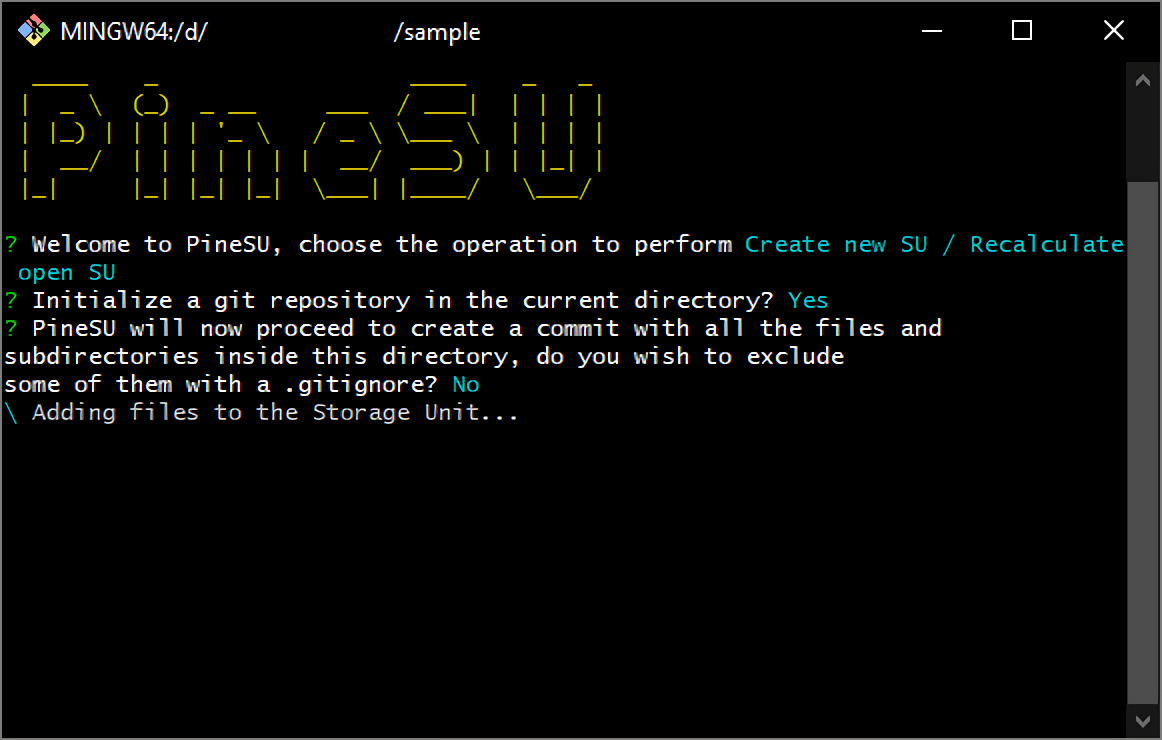
\includegraphics[width=0.9\textwidth]{Figures/calculating}
    \caption{\small{
    L'interfaccia di PineSU durante il calcolo.
    } % end small
    } % end caption
    \label{fi:calc}
\end{figure}


Una volta finito di calcolare ci verranno fatte domande sulla natura della Storage Unit come il suo nome,
la repository remota a cui si sincronizza, la sua descrizione, ecc\dots
Finite le domande, l'applicativo ci riporterà al menù principale.

\begin{figure}[H]
    \centering
    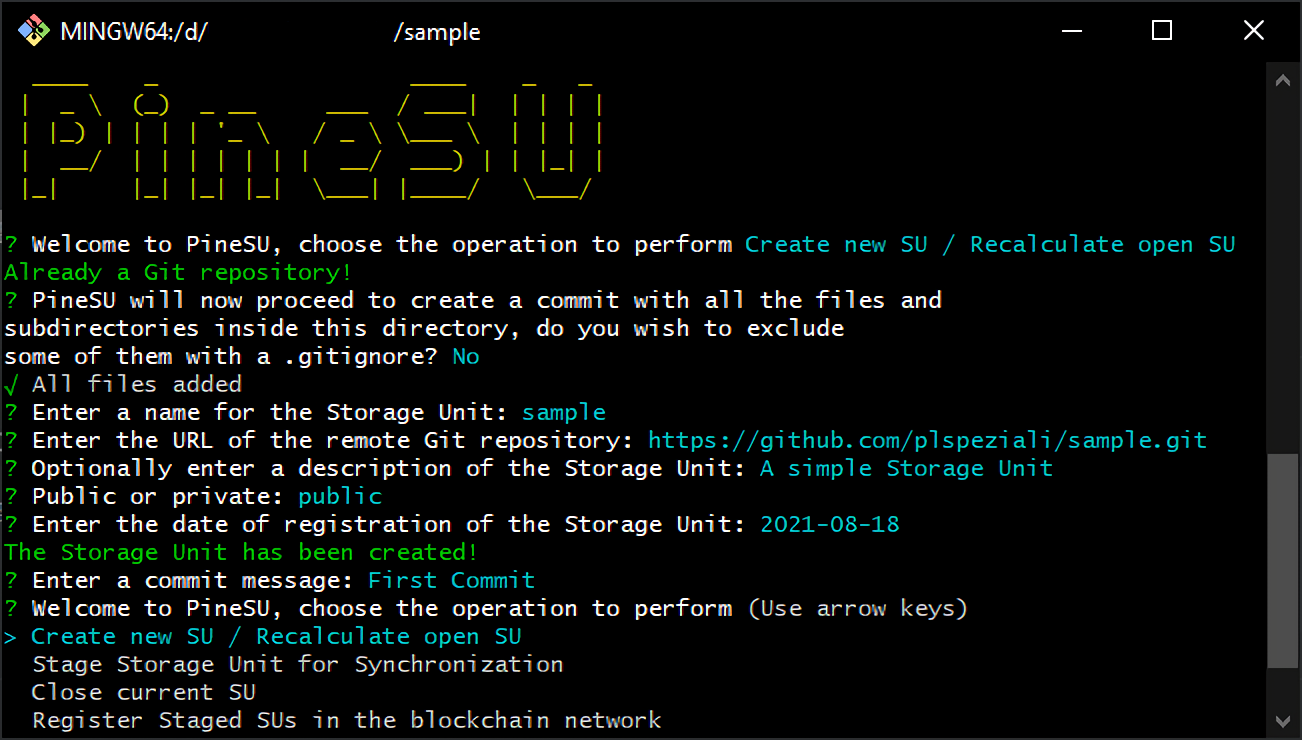
\includegraphics[width=0.9\textwidth]{Figures/doneCalculating}
    \caption{\small{
    L'interfaccia di PineSU appena terminata la fase di creazione.
    } % end small
    } % end caption
    \label{fi:dcalc}
\end{figure}

Al termine di entrambe le elaborazioni sulle due directory avremo alcune nuove aggiunte al loro interno:
una cartella .git (eventualmente, anche un file .gitignore) e un file .pinesu.json, quest'ultimo è
il descrittore JSON in cui sono salvate le informazioni che abbiamo inserito, gli hash calcolati e
lo stato di chiusura. Ecco, ad esempio, il file JSON di \emph{sample}:

\begin{lstlisting}[language=json,firstnumber=1]
{"name": "sample",
"remote": "https://github.com/plspeziali/sample",
"description": "A simple Storage Unit",
"visibility": "public",
"date": "2021-08-18",
"owner": "0xCF23544bFC002905532bD86bF647754A84732966",
"hash": "3837ec6fe66032ba593d227ee800a079c61a5853",
"filelist": [
    "first/astar.js:e09deffb3654301a9a8d20acc5a7091cda7039b6",
    "first/graph.js:53982e4feeaf1445434864b409014706e31da1cc",
    "graphCreator.js:c3b4338c33d6ea5a30b31c16defc7661a4ae767b",
    "second/priorityQueue.js:1cb66abaaafd6a7125ab7dac1d7e0fb1860da574",
    "second/third/main.js:1b8dad338691dead8edc66e7c01b8db6d834e3d8",
    "second/third/vertex.js:aa3fa9242ceec7062c7d84764e4068711e53c4e3",
    "first:75d936d52208d14c2cd571e0c595bc29e7d0e3a0",
    "second/third:2ec86afc483f3685893831dfe04b66620be690d2",
    "second:d6e51cdbe8a84cb3ba2c9cfdc2773a96b2401a59"
],
"closed": false }
\end{lstlisting}
\newpage

\section{Staging delle Storage Unit}

A questo punto vogliamo registrare le nostre Storage Unit aperte nella blockchain, 
occorre però prima inserirle negli Storage Group
(in questo caso solo in Open Storage Group).
Per effetturae questa operazione occorro solo selezionare l'opzione omonima
in entrambe le directory, nella nostra cartella d'installazione verrà
aggiornato il file \emph{merkles/storageGroup.json} con le informazioni delle nostre SU.

\begin{lstlisting}[language=json,firstnumber=1]
[ {
    "name": "sample",
    "hash": "3837ec6fe66032ba593d227ee800a079c61a5853",
    "path": "D:/Progetti/Tirocinio/sample",
    "closed": false
  },
  {
    "name": "secondSample",
    "hash": "7a61ed5e43cd436fb1f88895625a8193fdb9b3be",
    "path": "D:/Progetti/Tirocinio/secondSample",
    "closed": false
  } ]  
\end{lstlisting}
Questa è la lista delle foglie con cui calcoleremo l'effettivo Merkle Tree di OSG.

\section{Registrazione su Blockchain}